\Chapter{Modélisation par les vitesses de dérive}
\chaptermark{Les vitesses de dérive}
\begin{refsection}
Le deuxième chapitre de cette thèse concerne la modélisation du transport
(fortement) magnétisé par une approche basée sur les vitesses de dérive. Cette
méthode, élaborée dans le cadre de la recherche sur la fusion par
confinement magnétique, est implémentée dans TOKAM2D~\cite{Sarazin}, un code 
spécialement développé pour caractériser le transport dans le plasma de bord
des tokamaks.

Nous introduisons tout d'abord le code TOKAM2D et les hypothèses sur
lesquelles repose le modèle. Les équations de continuité et de
courant sont ensuite dérivées avec quelques précisions sur les approximations
choisies.
Dans une deuxième partie, nous présentons les évolutions du
modèle et les modifications entreprises sur le code pour lui
permettre décrire le transport dans des conditions caractéristiques aux plasmas
froids. Sont ainsi passées en revues :

\begin{itemize}
  \item l'inclusion de conditions aux limites
perpendiculaires
\item la prise en compte d'une géométrie quelconque pour le champ magnétique
\item l'ajout de l'équation d'énergie pour la
température électronique
\item la construction d'un modèle basé sur les vitesses de dérive pour les plasmas froids
\end{itemize}

Pour le dernier point, les équations sont redérivées en tenant
compte du transport collisionnel avec les neutres. Le modèle intègre de plus des
conditions aux limites de type gaine sur le courant et le flux de particules
dans la direction perpendiculaire au champ magnétique.



\section{Le code TOKAM2D}

\sectionmark{Le code TOKAM2D}
La première année de cette thèse a consisté à utiliser et modifier le
code {TOKAM2D}. Le but était alors de se familiariser avec les mécanismes du
transport magnétisé et les techniques développées pour la modélisation des
plasmas de Scrape-Off-Layer (SOL) afin
de pouvoir les appliquer au problème des sources d'ions. 

Le code TOKAM2D est un code fluide, quasineutre, qui décrit le transport
transverse en se basant sur l'approximation des vitesses de dérive (voir
\S~\ref{ApproximationsEqMvt}-\ref{vitessesDerive}). Il fut initialement
développé à l'Institut Méditerranéen Technologique de Marseille (IMTM) pour
étudier la turbulence générée par l'instabilité d'interchange qui résulte de
l'interaction entre le gradient de pression et la courbure du champ
magnétique~\parencite{Garbet}. C'est l'un des premiers codes à avoir opté pour
un forçage de la turbulence par un flux au lieu d'un gradient d'équilibre afin
de lever et de remettre en question l'hypothèse de séparabilité des échelles
entre l'équilibre et les fluctuations qui était utilisée auparavant.

Le code TOKAM2D a entre autre permis retrouver le caractère extrêmement
intermittent du transport dans la SOL et la longueur de décroissance du profil de densité que l'on
mesurait expérimentalement~\cite{SarazinPhD}. L'étude du modèle a ainsi aidé à
améliorer la compréhension du mécanisme de l'instabilité d'interchange,
notamment par l'analyse
du déclenchement à seuil de l'instabilité et la mise en évidence d'un transport
convectif turbulent, qui se caractérise par l'apparition de structures de
densité auto-organisées se propageant radialement sur de longues distances (des avalanches).

\subsection{Hypothèses du modèle}
Dans les conditions typiques de la SOL ($n_e\sim\,$10$^{19}$~m$^{-3}$,
$T_e\sim\,$70~eV), l'utilisation d'un modèle fluide est justifiée par la forte
collisionnalité du plasma : pour les ions, le libre parcours moyen
$\lambda_i=v_{\text{T}{i}}/\nu_{ei}$, de l'ordre du mètre, est très
inférieur à la longueur de connexion parallèle des lignes de champ
$L_\para\sim\,$100~m.

Le plasma est de plus très magnétisé $B\sim\,$1~T ; les fréquences
caractéristiques du transport transverse sont donc suffisamment lentes devant la
fréquence cyclotronique ionique pour nous placer dans le cadre de
l'approche par vitesses de dérive (cf. \S\ref{Introduction}\ref{vitessesDerive})
:

\begin{equation}
\omega\ll\omega_{ci}\Leftrightarrow
\varepsilon_\omega\equiv\frac{\omega}{\omega_{ci}}\ll 1
\end{equation}

D'un autre côté $\rho\indice{Li}$, le rayon de Larmor ionique, d'environ
1mm, est bien supérieur à la longueur de
Debye $\lambda_D$, de l'ordre de 10$^{-5}$~m, ce qui autorise à
considérer le plasma quasineutre dans son ensemble, avec des densités ionique
et électronique égales à $n$.
Le transport est alors décrit à travers l'évolution de la densité
électronique $n$ et du potentiel électrostatique $\Phi$ en résolvant l'équation
de continuité des électrons ainsi que l'équation de conservation du courant. Les
températures électronique
$T_e$ et ionique $T_i$ sont supposées constantes, avec un rapport $\tau=T_i/T_e$.

Enfin, le problème est réduit de trois à deux dimensions sur la base de l'hypothèse
flûte, qui suppose une propagation instantanée des fluctuations le long des
lignes de champ : les conditions aux limites parallèles, dérivées du critère de
Bohm, deviennent des termes sources après l'intégration des équations le long
des lignes de champ magnétique.

\begin{figure}[!htbp]
\centering
    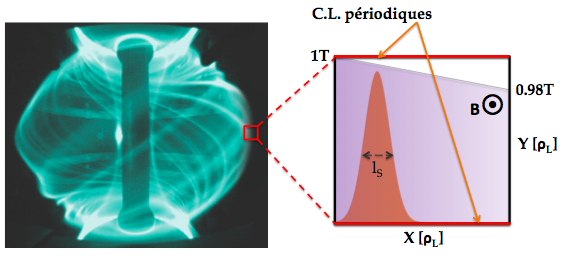
\includegraphics[width=0.9\textwidth]{figures/2-tokamSimDomain.png}
    \caption{La région simulée est située à la frontière du plasma confiné,
    au niveau de la séparatrice, et dans le plan poloïdal médian.}
    \label{2-figTokamGeom}
\end{figure}

La figure~\ref{2-figTokamGeom} montre la zone simulée. La SOL est représentée dans le plan
poloïdal (perpendiculaire à la direction toroïdale)
en géométrie slab\footnote{Dans cette approche simplifiée, l'enroulement des
lignes de champ autour des surfaces magnétiques est supposé suffisamment
faible pour que l'on puisse assimiler la direction parallèle ($z$) à la
direction toroïdale. Dans ces conditions, le gradient transverse d'une
grandeur $f$ par rapport à l'angle poloïdal $\theta$ peut être approximé avec
les coordonnées normalisées par la dérivée $\partial_y$ en supposant $r\approx
a$ :
$$\frac{\rho_{Li}}{r}\partial_\theta f(x,y)\approx\partial_y
f(x,y)$$
ce qui constitue l'approximation slab. Ces
coordonnées n'intègrent donc pas les effets de courbure géométrique.}, ie.
avec $x\equiv(r-a)/\rho_{Li}$ et $y\equiv a\theta/\rho_{Li}$ les coordonnées
transverses au champ magnétique
(cf.~\S\ref{ApproximationsEqMvt}-\ref{1-vitessesDerive}), normalisées par le rayon de Larmor ionique.

La séparatrice est modélisée par un terme source entrant de particules, de profil gaussien :

\begin{equation}
\mathcal S=\mathcal{S}_0 \exp[(x-x_\mathcal{S})^2/l_\mathcal{S}^2]
\end{equation}

Le terme source sépare la zone
simulée en deux régions :

\begin{itemize}
  \item une région stable à gauche
  de la source, qui peut représenter la SOL côté champ fort (High Field
  Side (HFS), entre le centre du tokamak et le plasma de c\oe ur). Dans cette
  région, la courbure magnétique est favorable à la stabilité vis-à-vis de l'instabilité
  d'interchange $\nabla 1/B\cdot\nabla N>0$
  \item une région sujette à l'instabilité d'interchange à
  droite de la source, qui modélise la SOL côté faible champ (Low Field Side
  (LFS), entre le plasma de c\oe ur et la paroi extérieure du tokamak)
 \end{itemize}
 
Dans la version initiale de TOKAM2D, le domaine de simulation a été choisi
bipériodique pour permettre un traitement dans l'espace
de Fourier.

\subsection{Dérivation des équations}
\subsubsection{Équation de conservation de la matière}
La densité $n$ du plasma est contrôlée par l'équation de continuité des
électrons\footnote{Pour modéliser le transport dans les plasmas froids, en
l'absence de champ magnétique, l'habitude est plutôt de calculer la densité
plasma à partir de l'équation de continuité des ions, ceux-ci ayant une
dynamique bien plus lente que les électrons et des conditions aux limites
bien définies au niveau des parois ou des gaines. Ce choix permet en plus de
traiter les plasmas multi-espèces sans difficulté.

Dans les plasmas d'hydrogène fortement magnétisés caractéristiques des tokamaks,
le transport dans la direction transverse au champ magnétique est
essentiellement dû à la dérive $\mathbf E\times\mathbf B$, identique pour les
ions et les électrons. Suivre la population électronique à la place de la
population ionique permet alors de négliger le terme d'inertie avec plus de
légitimité (ce dernier étant critique pour les ions dans le cas de plasmas
froids basse-pression).}.
En notant $\mathcal{S}$ un
terme source modélisant les particules provenant du plasma de
c\oe{}ur (c'est le terme qui constitue le forçage par le flux de la turbulence),
l'équation de continuité s'écrit :

\begin{equation}
\label{2-ContinuiteElectrons}
\partial_t n + \nabla\cdot(n\mathbf{u}) = D_\perp\nabla^2_\perp n + \mathcal{S}
\end{equation}

avec $\mathbf u$ la vitesse fluide électronique. Le terme diffusif, de
coefficient $D_\perp$, est ajouté pour contrôler l'erreur du schéma d'advection et le stabiliser. Il s'inspire de la description
dite "classique" du transport transverse, qui consiste à approximer l'effet des
collisions coulombiennes par une diffusion de fréquence caractéristique
$\nu_{ei}$ et de pas caractéristique $\rho_{L}$. Le coefficient
$D_\perp\sim\nu_{ei}\rho_{Li}^2$ varie peu dans l'ensemble du plasma et présente
une valeur typique de 10$^{-2}\,$m$^2$.s$^{-1}$.

La divergence du flux d'advection peut se décomposer suivant les directions
parallèle et perpendiculaires. En se souvenant que le flux de matière
transverse est essentiellement issu de l'advection par la vitesse de dérive électrique
(cf.~\S~\ref{ApproximationsEqMvt}-\ref{vitessesDerive}), \eqref{2-ContinuiteElectrons}
se développe en :

\begin{equation}
\label{2-ContinuiteElectrons2}
\partial_t n + \nabla_\para(nu_{\para}) +
\mathbf{u}_E\cdot\nabla_\perp n = D_\perp\nabla^2_\perp n + \mathcal{S}
\end{equation}

En substituant l'expression de la vitesse de dérive électrique
(\eqref{1-eqVitessesDerive}) dans le terme d'advection
$\mathbf{u}_E\cdot\nabla_\perp n$, celui-ci peut s'écrire en utilisant la
notation du crochet de Poisson $[n,\Phi]=\mathbf{b}.(\nabla_\perp
n\times\nabla_\perp\Phi)$, où $\Phi$ est le potentiel
électrique dont dérive le champ électrique $\mathbf E=-\nabla\Phi$. C'est la
forme que prend toute advection d'un champ scalaire par une vitesse de dérive
$\mathbf{v}_\text{D}=\nabla H\times\mathbf{B}/B^2$, où $\nabla H$ est la force
à l'origine de la dérive. L'équation de continuité pour les électrons s'écrit alors :

\begin{equation}
\label{2-eqContinuiteFinale}
\partial_t n + \nabla_{\para}(nu_{\para}) =
\frac{1}{B}\left[n,\Phi\right] + D_\perp\nabla^2_\perp n + \mathcal{S}
\end{equation}

Le terme non-linéaire $[n,\Phi]$ est l'un des éléments moteur du modèle
d'interchange. Couplant la densité au potentiel électrique, il opère un
transfert d'excitation des composantes radiales des fluctuations à leurs
composantes poloïdales et réciproquement. Les termes de flux parallèle et de
diffusion sont stabilisant, ils tendent à
amortir les fluctuations et donc à homogénéiser le système.

\subsubsection{Équation de conservation du courant}
L'équation de conservation du courant s'obtient en soustrayant l'équation de
continuité des électrons à celle des ions. La vitesse de dérive électrique
$\mathbf{u}_E$, indépendante de la masse et de la charge des particules,
est identique pour les deux espèces et ne transporte aucun courant. 
La conservation du courant se résume donc à un équilibre entre le courant
parallèle $\mathbf{j}_\para$ et les courants transverses diamagnétique
$\mathbf{j}_*$ et de polarisation $\mathbf{j}_p$ à travers leur
divergences:

\begin{equation}
\label{EqCourant1}
\nabla\cdot\left(\mathbf{j}\right) = 
\nabla\cdot\left(\mathbf{j}_\para+\mathbf{j}_*+\mathbf{j}_p\right)
= 0
\end{equation}

La divergence du courant diamagnétique, dans un plasma isotherme, donne un
crochet de Poisson entre la densité et la courbure du champ magnétique :

\begin{equation}
\nabla\cdot\mathbf{j}_*=
\nabla_\perp\cdot\left(\nabla_\perp\left(
P_i+P_e\right)\times\mathbf{B}/B^2\right) =
eT_e(1+\tau)\left[n,B\puissance{-1}\right]
\end{equation}

La vitesse de polarisation étant
proportionnelle à la masse des particules \eqrefp{1-vitessePol}, on ne
retient dans l'expression du courant que la contribution ionique :

\begin{equation}
\mathbf{j}_p\sim
en\mathbf{u}^i_p=-\frac{nm_{i}}{B^2}\frac{\text{d}\nabla_\perp \Phi}{\text{dt}}
\end{equation}

En exprimant la dérivée totale de
façon eulérienne, la divergence du courant de polarisation devient :

\begin{equation}
\nabla\cdot\mathbf{j}_p\sim\nabla\cdot\left({e}n\mathbf{u}^i_p\right)\equiv
-\nabla_\perp\cdot\left(\frac{nm_{i}}{B^2}\left(\partial_{t} -
\nu_\perp \nabla_\perp^2 +
\mathbf{u}\cdot\nabla_\perp\right)\nabla_\perp \Phi\right)
\end{equation}

La contribution d'effet visqueux est rajoutée, pour les même raisons que
$D_\perp$, à travers la viscosité ionique perpendiculaire $\nu_\perp$.
De manière similaire à \eqref{2-ContinuiteElectrons2}, seule l'advection par la
vitesse de dérive électrique est considérée dans la divergence : 
$\nabla\cdot\left(\mathbf{u}\,\nabla_\perp^2 \Phi\right)
\approx\nabla\cdot\left(\mathbf{u}_E\,\nabla_\perp^2 \Phi\right)$.
En insérant l'expression des dérives, \eqref{EqCourant1} se réécrit :

\begin{equation}\begin{split}
\label{EqCourant2}
\nabla_\para j_\para +
eT_e(1+\tau)\left[n,B\puissance{-1}\right] +
\nabla_\perp\cdot\left(-\frac{nm_{i}}{B^2}\left(\partial_{t}\nabla_\perp \Phi - \nu_\perp \nabla_\perp^3 \Phi \right)\right) \\+
\nabla_\perp\cdot\left(-\frac{nm_{i}}{B^2}\mathbf{u}_E\cdot\nabla_\perp^2
\Phi\right)=0
\end{split}
\end{equation}

Diverses considérations sur l'importance relative des termes contenus dans
\eqref{EqCourant2} (reliées aux hypothèses d'ordering
et aux variations de champ magnétique) sont développées dans la thèse de Yannick
Sarasin~\cite{SarazinPhD}. En effectuant un changement de variable
$\Omega=\nabla_\perp^2\Phi$, où $\Omega$ symbolise une vorticité\footnote{La
vorticité d'un écoulement est généralement définie comme le rotationnel de sa vitesse. Dans la SOL, le champ de vitesse correspond essentiellement à la dérive ExB, ce qui donne pour un champ magnétique constant de 1T : 
$\nabla\times\mathbf{v}\sim\nabla\times\mathbf{u}_E=\nabla\times(\mathbf{E}/B\times\mathbf{b})\equiv-\nabla_\perp^2
\Phi=\Omega$ }, \eqref{EqCourant2} se transforme en une équation simplifiée dite
de vorticité:

\begin{equation}\begin{split}
\label{2-eqCourantFinale}
\nabla_\para{j}_\para +
eT_e(1+\tau)\left[n,B\puissance{-1}\right] =\\
\frac{nm_i}{B^2}\left(\partial_{t}\Omega - \nu_\perp
\nabla_\perp^2\Omega+
B\puissance{-1}\left[\Phi,\Omega\right]\right)
\end{split}
\end{equation} 

 Dans le système d'équations
 \eqref{2-eqContinuiteFinale}~--~\eqref{2-eqCourantFinale}, seules restent
 inconnues la vitesse parallèle électronique  et le courant parallèle. Le
 système se referme alors en moyennant les équations le long de la
 direction parallèle. 

\subsection{Système moyenné et normalisation}
\label{2-flute}
\subsubsection{Réduction 2D}

 L'hypothèse flûte, qui s'appuie sur des observations
expérimentales\footnote{Des mesures expérimentales ont montré que le vecteur
d'onde parallèle des fluctuations électrostatiques était très petit devant la
longueur de connexion parallèle $L_\para$\parencite{Wootton}}, consiste à
considérer les fluctuations constantes le long des lignes de champ. Toute
grandeur $f(x,y,z)$ vérifiant l'hypothèse flûte est donc indépendante de la
direction parallèle $z$ et sa moyenne est égale à la fonction elle-même :

\begin{equation}
\left<f(x,y,z)\right>_\para\rightarrow f(x,y)
\end{equation}

En supposant que la densité $n$ et le potentiel $\Phi$ vérifient cette hypothèse
flûte, le passage des équations
\eqref{2-eqContinuiteFinale}~--~\eqref{2-eqCourantFinale} à la moyenne laisse la plupart des termes inchangés.

Les divergences parallèles du flux et du
courant font naturellement apparaître
les conditions aux limites de gaine issue du critère de Bohm
(cf.~\S~\ref{Introduction}-\ref{1-gaine}) :

\begin{align}
\left<\nabla_\para
nu_\para\right>_\para&=\frac{nc_s}{L_\para}\exp(\Lambda-(\Phi-\Phi_\text{w})/T_e)
\\
\left<\nabla_\para
j_\para\right>_\para&=\frac{enc_s}{L_\para}\left(1-\exp(\Lambda-(\Phi-\Phi_\text{w})/T_e)\right)
\end{align}

où $c_s=\sqrt{eT_e/m_i}$ est la vitesse acoustique
ionique, $\Lambda=T_{e}\ln({m_{i}/2\pi m_{e})/2}$ est le
potentiel flottant et $\Phi-\Phi_\text{w}=\Delta \Phi$ représente la
différence de potentiel entre le plasma et la paroi. 

La moyenne sur le terme de courbure est plus délicate à obtenir et doit tenir
compte de l'enroulement des lignes de champ magnétique.
Dans~\parencite{Garbet}, Xavier Garbet détermine un coefficient de courbure
moyen $g_\perp\propto\partial_xB^{-1}$ (qui se mesure en T$^{-1}$.m$^{-1}$) tel
que :

\begin{equation}
\left<eT_e(1+\tau)\left[n,B^{-1}\right]\right>_\para=eT_eg_\perp\partial_yn
\end{equation}

comme ce coefficient est positif, le signe du terme déstabilisant
de l'interchange ne dépend plus que du sens du gradient
radial de densité. Le mécanisme d'interchange sera donc stable à gauche de la
source et le transport turbulent ne se développera que du côté droit de la zone
de simulation, où le gradient radial moyen de densité est négatif.
Avec ces expressions, le système d'équations \eqref{2-eqContinuiteFinale}~--~\eqref{2-eqCourantFinale} devient :

\begin{align}
\label{2-eqContinuiteMoyenne}
&\partial_t n + \frac{nc_s}{L_\para}e^{\Lambda-\Delta \Phi/T_e} =
\frac{1}{B}\left[n,\Phi\right] + D_\perp\nabla^2_\perp n + \mathcal{S}\\
&\partial_{t}\Omega - \nu_\perp
\nabla_\perp^2\Omega+
\frac{1}{B}\left[\Phi,\Omega\right]=\frac{ec_sB^2}{m_iL_\para}\left(1-e^{\Lambda-\Delta
\Phi/T_e}\right) -\frac{B^2}{m_i}eT_eg_\perp\partial_y\ln n
\label{2-eqCourantMoyenne}
\end{align}
 
\subsubsection{Normalisation des équations}

Considérons maintenant le champ magnétique et la température constants en espace
et en temps :
\begin{equation}
B=B_{\indice{0}}=1\,\text{T~~~~~~~et~~~~~~~}eT_e=eT_0=1\,\text{eV}
\end{equation}
et supposons les
ions froids $T_i=\,$0.
Pour faire apparaître les grandeurs caractéristiques du système et simplifier
l'écriture des équations, les différents termes sont adimensionnés à
l'aide de ces deux constantes. Le temps est normalisé à l'inverse de la
fréquence cyclotronique ionique :

\begin{equation}
t = \overline{t}\:\omega_{ci}\puissance{-1} =
\overline{t}\:\frac{m_i}{eB\indice{0}}
\end{equation}

Les longueurs et vitesses sont alors logiquement normalisées par le rayon de
Larmor et la vitesse de Bohm :

\begin{eqnarray}
x = \overline{x}\:\rho_{Li} =
\overline{x}\:\frac{m_ic_s}{eB\indice{0}} &
et &
v=\overline{v}c_s=\overline{v}\sqrt{\frac{eT\indice{0}}{m_i}}
\end{eqnarray}

Nous définissons de plus les variables adimensionnées du modèle, la densité
$\text{N}$, le potentiel électrostatique $\overline{\Phi}$ (pour lequel nous
garderons la même notation, ie. sans la barre, dans le reste du chapitre) et la
vorticité $\text{W}$ par :

\begin{eqnarray}
n = n_{\indice{0}}\text{N} \text{~~~~~~~} \Phi=\frac{\overline{\Phi}
T\indice{0}}{e}
\text{~~~~~~~} \Omega=\frac{\text{W} T\indice{0}}{e\rho_L^2}
\end{eqnarray}

Avec cette normalisation, on
réécrit le système d'équations
(\eqref{2-eqContinuiteMoyenne}--\eqref{2-eqCourantMoyenne}) sous la forme :

\begin{align}
\label{2-eqContinuiteNorm}
&\partial_t \text{N}
= \left[\Phi,\text{N}\right] -\sigma \text{N}e^{\Lambda-\Delta\Phi}
 + D\nabla^2 \text{N} + \mathcal{S}
\\
\label{2-eqCourantNorm}
&\partial_{t}\text{W} = 
\left[\Phi,\text{W}\right]
+\sigma\left(1-e^{\Lambda-\Delta\Phi}\right) 
-g\partial_y\log\text{N}
+\nu\nabla_\perp^2\text{W}
\end{align}
 
Les coefficients de diffusion $D$ et de viscosité $\nu$ sont normalisés au
coefficient de Bohm $D_B=\rho_{Li}c_s$\footnote{Le coefficient normalisé de
diffusion $D$ peut aussi se lire comme le ratio entre la fréquence des
collisions coulombiennes et la fréquence cyclotronique ionique :
$$D=\frac{D_\perp}{D_B}=\frac{\nu_{ei}\rho_{Li}^2}{\rho_{Li}c_s}=\frac{\nu_{ei}}{\omega_{ci}}$$
}.
Du côté droit, nous interprétons $\sigma=\rho_{Li}/L_\para$ comme une
conductivité de gaine. Du fait de sa faible valeur $\sigma\sim\,$10$^{-5}$, elle
limite les pertes en courant parallèle au niveau des parois (limiteur),
permettant à l'instabilité de se développer. Ce terme régule le potentiel
électrostatique et amortit les fluctuations, en ramenant constamment le
potentiel plasma à $\Lambda$, le potentiel flottant.

Le quatrième terme de~\eqref{2-eqCourantNorm}, issu de la divergence
du courant diamagnétique, contient l'élément déstabilisant de
 l'instabilité d'interchange. La force générée par la courbure du champ
 magnétique joue dans un tokamak le même rôle que la gravitation dans
 l'instabilité de Rayleigh-Taylor : dirigée vers l'extérieur du tore, elle 
 résulte en une poussée du fluide le plus dense sur le fluide le plus léger. 
 
 Le terme non linéaire $[\Phi,\text{W}]$ dérive du courant de polarisation.
 Fondamentalement relié à l'inertie des ions, il advecte les structures de
 potentiel dans la direction de la dérive électrique.
 

\subsection{Le transport transverse dans la SOL}

Le système d'équations
adimensionnées (\eqref{2-eqContinuiteNorm}--\eqref{2-eqCourantNorm}) est un
modèle 2D minimal pour étudier l'instabilité d'interchange qui se développe dans
la SOL des tokamaks. La figure~\ref{2-CartesBase} montre les solutions obtenues
par TOKAM2D pour une simulation typique de plasma de bord, dont les paramètres
sont donnés dans le tableau~\ref{2-TokamParam} :

\begin{table*}[!htbp]
\footnotesize\centering
\ra{1.3}
\begin{tabular}{@{}lcccccc@{}}\toprule
Définition&&Paramètre&&Expression&&Valeur\\
\midrule 
Nombre de maille&&$N_x$, $N_y$ && - && 256\\
Taille du domaine&&$L_x$, $L_y$ &&$L_x$, $L_y$ /$\rho_{Li}$ && 256\\
Intensité source&&$\mathcal{S}_0$ &&
$\mathcal{S}_0$/$n_0\omega_{ci}$
&& 10$^{-2}$\\
Profil source&& $x_\mathcal{S}$,
$l_\mathcal{S}$ && $\exp[(x-x_\mathcal{S})^2/l_\mathcal{S}^2]$
&& 64,32\\
Coefficient de courbure&&$g$ &&
$(\rho_{Li}(1+\tau)/R_0)\sin\text{c}(\Delta\theta)$\footnotemark &&
5.10$^{-4}$\\
Conductivité de gaine&&$\sigma$ &&
$\rho_{Li}/L_\para$ &&
10$^{-5}$\\
Coefficient de diffusion, viscosité&&$D,\nu$ &&
$D_\perp,\nu_\perp/D_B$ &&
10$^{-2}$\\
\bottomrule
\end{tabular}
\caption{Tableau présentant les paramètres du modèle et
leur valeur typique.}\label{2-TokamParam}
\end{table*}
\footnotetext{L'expression provient de \parencite{SarazinPhD}. On note
$\sin\text{c}(\Delta\theta)\sim\sin(\Delta\theta)/\Delta\theta$.
$\Delta\theta$ représente l'écartement du limiteur par rapport à l'angle
poloïdal de symétrie $\theta_0=0$}

\begin{figure}[!htbp]
    \centering
    \subfigure[]{\label{2-CarteDensiteBase}
    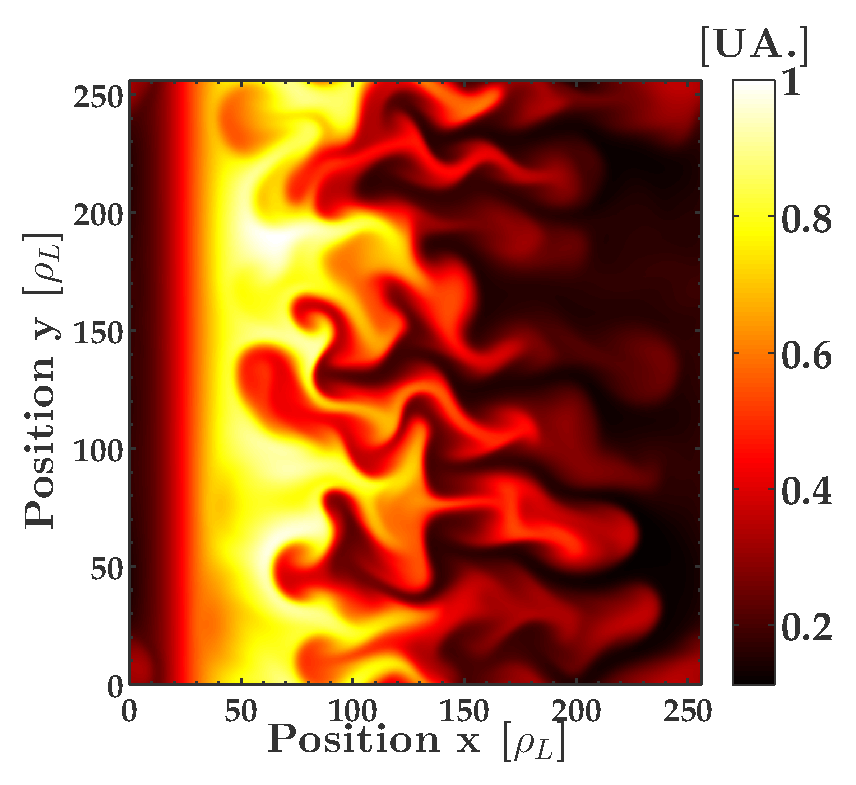
\includegraphics[height=6cm]{figures/2-CarteDensiteBase.eps}}
    \subfigure[]{\label{2-CartePotentielBase}
    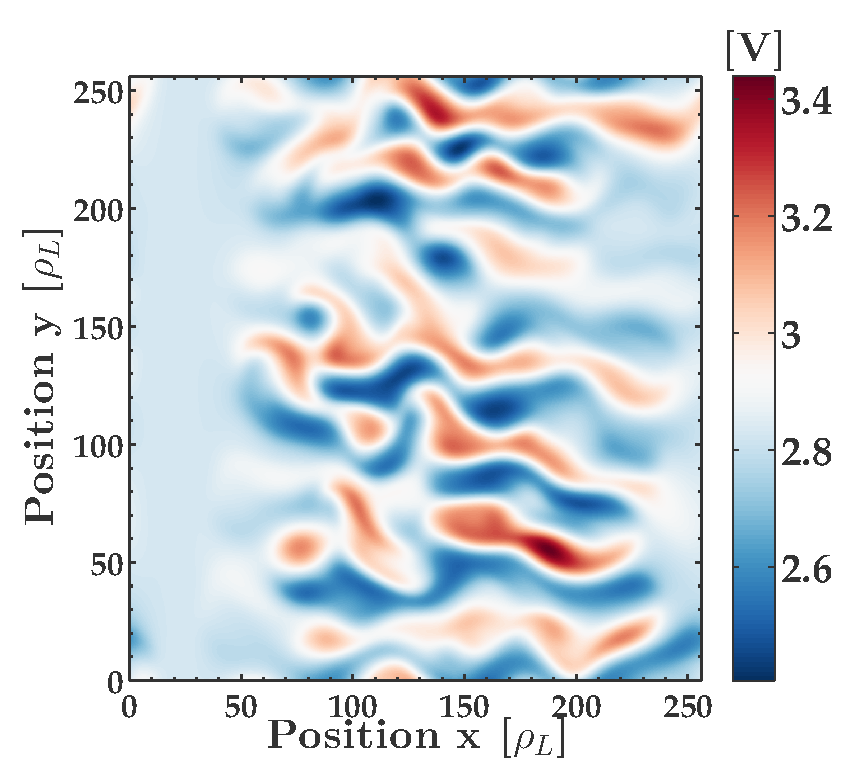
\includegraphics[height=6cm]{figures/2-CartePotentielBase.eps}}
    \caption{Cartes de la densité~\subref{2-CarteDensiteBase}~~et du potentiel
    électrostatique~\subref{2-CartePotentielBase}. Le profil du terme source
    $\mathcal{S}$ est représenté en gris sur la carte de densité.
    }
    \label{2-CartesBase}
\end{figure}

A gauche, le plasma est stable. A droite, le transport est dominé par l'instabilité d'interchange : de
forts flux de densité, des avalanches, traversent le domaine par intermittence.
Les fronts, qui peuvent se propager sur plusieurs centaines de
$\rho_{Li}$, augmentent considérablement la largeur de la SOL.
Les avalanches sont advectées par le champ électrique qui se créé entre les
structures de potentiel, dont la taille dans la direction $y$ est
typiquement de l'ordre de la dizaine de $\rho_{Li}$.
Un équilibre est atteint (la densité totale et le profil radial moyen
n'évoluent plus) quand les pertes parallèles égalent le transport radial moyen.

A l'équilibre, la nature de ce transport turbulent peut être
caractérisée statistiquement par des fonctions de distribution en probabilités
(PDF pour Probability Distribution Function) des différentes valeurs. Les PDF
de la densité et du flux radial sont présentées sur la figure~\ref{2-PDFBase} : 

\begin{figure}[!htbp]
    \centering
    \subfigure[]{\label{2-TokamPDFDensite}
    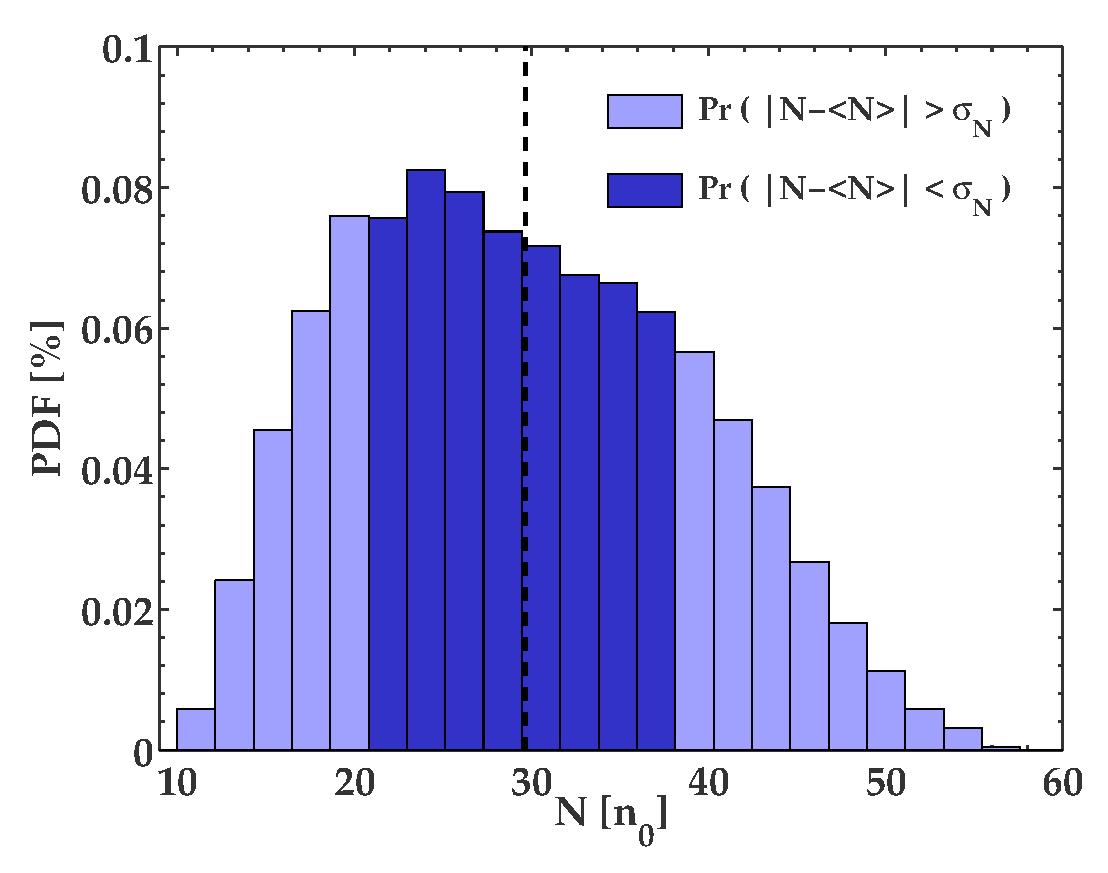
\includegraphics[width=0.45\textwidth]{figures/2-TokamPDFDensite.eps}}
    \subfigure[]{\label{2-TokamPDFFlux}
    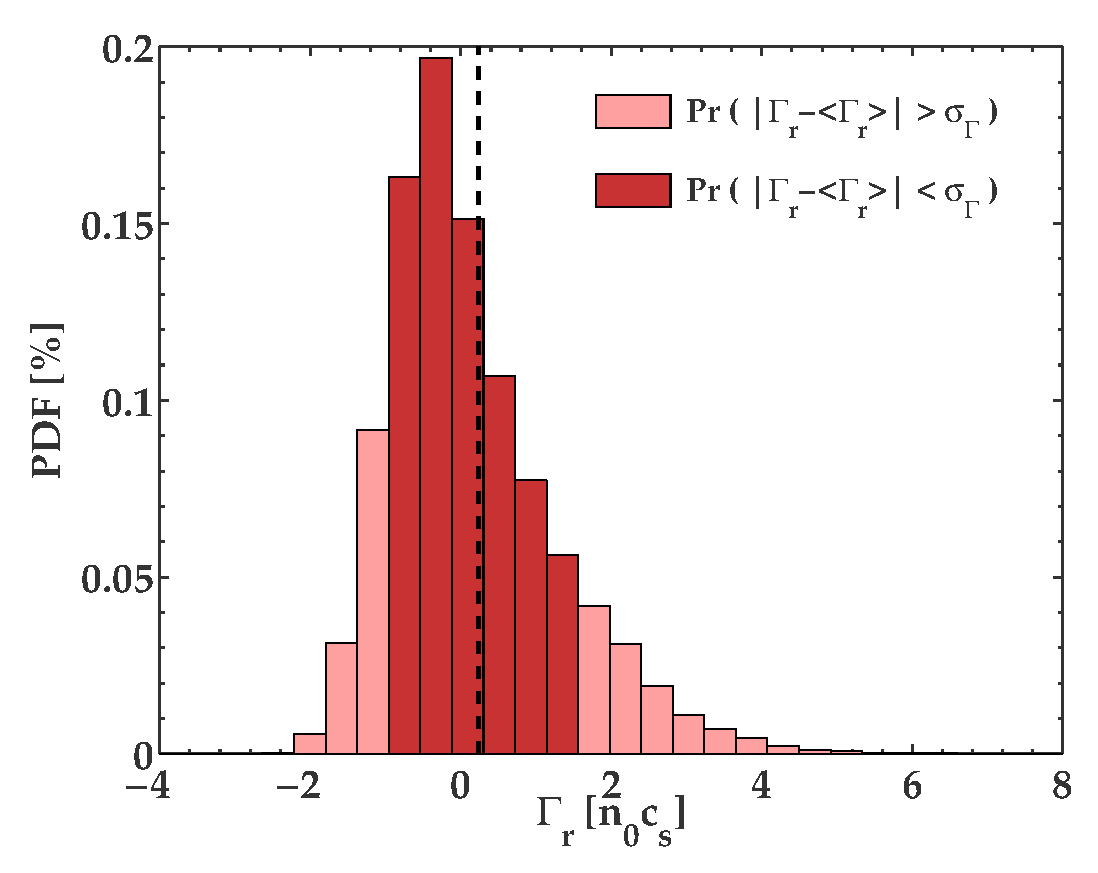
\includegraphics[width=0.45\textwidth]{figures/2-TokamPDFFlux.eps}}
    \caption{Fonction de distribution de probabilité pour la
    densité~\subref{2-TokamPDFDensite}~~et le flux
    radial~\subref{2-TokamPDFFlux}~. La moyenne est repérée par le trait en
    pointillé et l'écart type est montré en couleur plus foncée.}
    \label{2-PDFBase}
\end{figure}

Les PDF
sont calculées au milieu du domaine, à $x=\,$128$\,\rho_{Li}$, sur un
échantillon statistique de 2000 pas de temps et de 256 positions
poloïdales. La PDF donne en pourcentage la répartition globale des valeurs
que peut prendre la quantité et permet de quantifier l'importance des fluctuations.

Sur ces PDF, on voit par exemple que la densité et le flux radial sont le plus
souvent inférieurs à leur moyenne, et que des évènements plus
importants, de 3 à 4 fois l'écart type, les avalanches, peuvent apparaître. Bien
que les avalanches donnent l'impression d'un transport radial
important dirigé dans le sens des $x$ croissants, ces PDF
montrent que les densités et les flux statistiques les plus probables 
correspondent aux trous de plasmas qui remontent le gradient de densité. Le flux
moyen, résultant de la somme de ces évènements, n'est donc que légèrement
positif.

Dans cette partie, nous avons présenté le modèle de base et le type
de solutions que calculait TOKAM2D. Nous allons maintenant détailler les
modifications qui lui ont été apportées lors de la première année de ce travail
de thèse.

\section{Vers une description des sources d'ions}

Le modèle de TOKAM2D, dans la version que nous venons de présenter, n'est pas
directement applicable aux plasmas des sources d'ions. En effet dans
ces plasmas :

\begin{itemize}
	\item l'influence des parois sur le transport est primordiale. Des conditions
	aux limites périodiques, si elles sont acceptables dans le cadre de l'étude de
	l'instabilité d'interchange, ne peuvent pas représenter le champ électrique
	ambipolaire qui résulte de la chute de potentiel dans la prégaine
	\item le champ magnétique peut être
	totalement absent de certaines régions du plasma et présenter de forts
	gradients à l'entrée des zones magnétisées
	\item l'ionisation, processus contrôlant le bilan de particules, est fortement
	dépendante de la température électronique. Un modèle isotherme est donc
	intrinsèquement inadapté pour capturer la physique des sources d'ions
	\item le champ magnétique, de bien plus faible
	intensité, ne confine pas les ions qui ont en général un rayon de Larmor
	supérieur aux dimensions de la source
	\item la dynamique des espèces est dominée par la perte de
	quantité de mouvement liée aux collisions avec le gaz. La
	prise en compte du terme collisionnel dans l'équation du mouvement est
	alors primordiale.
\end{itemize}

Dans cette partie, nous présentons les évolutions successives du modèle pour
tenir compte des trois premiers points. 
Si les simulations de
cette version complétée de TOKAM2D ne correspondent pas encore aux plasmas
froids des sources d'ions, elles seront tout de même éclairantes sur le type de
transport qui se met en place dans des configurations de type filtre magnétique
et colonne de plasma pour des cas limites de notre étude, ie. où le plasma est
totalement ionisé et très magnétisé. La levée de ces deux hypothèses,
qui n'est possible qu'en incluant l'interaction avec les atomes neutres,
requiert une réécriture plus en profondeur du modèle, ce qui fait l'objet de la
partie suivante.

Dans le cadre de la recherche sur la fusion, cette refonte de TOKAM2D a tout
d'abord permis de vérifier les approximations choisies dans la description de
l'interchange du modèle original. Mais plus intéressant, les nouvelles
fonctionnalités développées dans le code ont donné lieu à des études sur
le transport du courant dans une géométrie radialement
non-périodique~\parencite{Futtersack} et sur l'influence de la température
électronique~\parencite{Moulton}.

\subsection{Étude sur les conditions aux limites}
	
	Lors de l'étude du mouvement des fluides, le type d'écoulement qui se
	forme est toujours fortement dépendant de la géométrie du système et des conditions aux limites
	imposées par l'environnement. Cette considération est aussi vraie dans le
	cas des plasmas dont l'évolution est totalement contrôlée par l'interaction
	avec les parois. Celle-ci est décrite par la théorie classique des gaines qui, 
	en nous donnant directement accès à la valeur des flux et des courants à la
	frontière du plasma, nous fournit des conditions aux limites concrètes
	reflétant la réalité physique.
	
	En présence d'un champ magnétique, le critère de Bohm reste valide le long
	des lignes de champ sur les parois du limiteur. Cependant, dans la direction
	perpendiculaire, aucune théorie équivalente n'a été dérivée. Le système devant
	tout de même être refermé, cette absence de théorie implique dans la
	construction des modèles un choix arbitraire de conditions aux limites, pas
	toujours sans conséquence.
	
	Les conditions aux limites ont été implémentées dans TOKAM2D de façon très
	souple afin de pouvoir choisir entre différentes combinaisons :
	
	\begin{equation}
	\label{2-BC}
		\alpha \partial^2_{x}\chi + \beta \partial_{x}\chi + \gamma \chi =
		\delta
	\end{equation}
	
	$\chi$ pouvant représenter la densité, le potentiel ou la vorticité. Par
	exemple, à l'aide de l'expression~\ref{2-BC}, le quadruplet
	\{0,0,$\gamma$,$\delta$\} définit une condition aux limites de Dirichlet, et
	\{0,$\beta$,0,$\delta$\} une condition aux limites de Neumann, toutes
	combinaisons étant possibles.
	Nous présentons ici une comparaison entre les résultats donnés par des
	conditions aux limites bi-périodiques, implémentées dans la version initiale de
	TOKAM2D, et ceux calculés avec des conditions aux limites absorbantes dans la
	direction radiale, que nous définissons par trois critères :
	
	\begin{itemize}
	  \item les particules sont perdues dans la gaine et aucun flux ne peut
	  provenir des parois 
	  \begin{equation}
	  	\Gamma_\text{N}\cdot\mathbf n\ge0
	  \end{equation}
	  \item Le
	potentiel est fixé au potentiel flottant, interdisant aux
	courants de sortir dans la direction transverse
	\begin{equation}
	  	\Phi(0,y)=\Phi(L_x,y)=\Lambda
	  \end{equation}
	\item La vorticité est totalement amortie au contact de la gaine 
	\begin{equation}
	  	W(0,y)=W(L_x,y)=0
	  \end{equation}
	\end{itemize}
	
	
\begin{figure}[!htbp]
\centering
    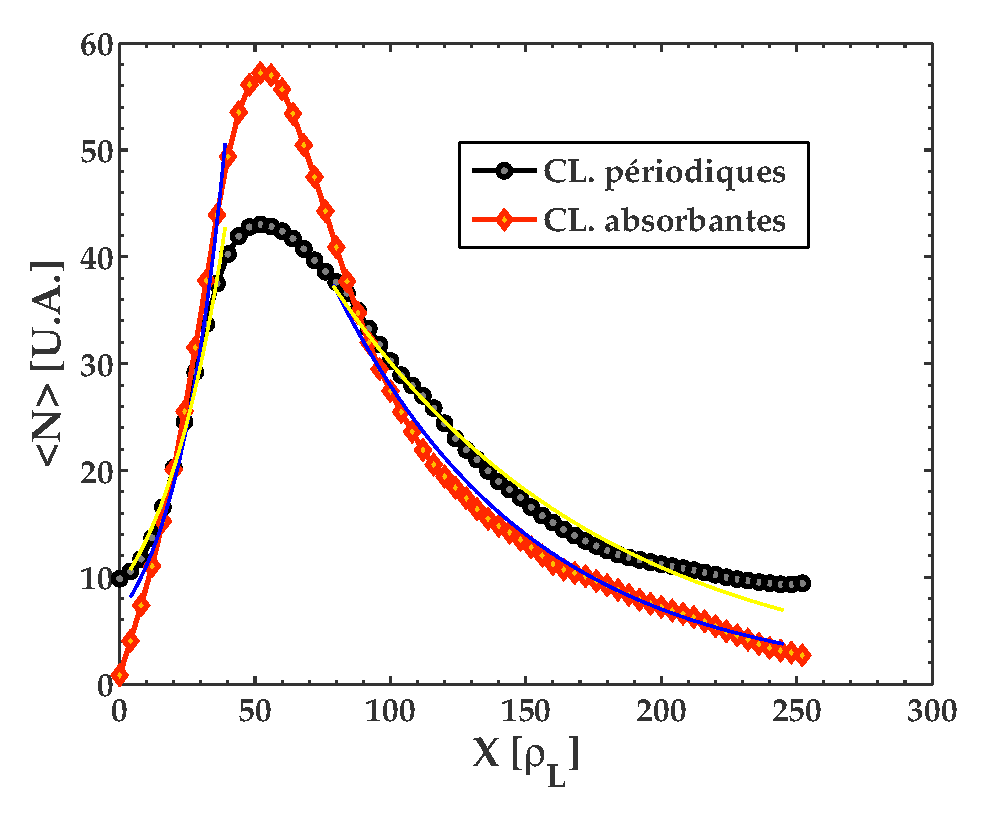
\includegraphics[width=8cm]{figures/2-profileDenNoLimit.eps}
    \caption{Profils radiaux (moyennés dans la direction poloïdale) de densité
    pour un cas périodique et un cas absorbant
    (non-périodique radialement)\label{2-profileDenNoLimit}.}
\end{figure}
	La figure~\ref{2-profileDenNoLimit} montre les profils de densité, moyennés
	dans la direction poloïdale, des deux simulations.
	Dans le cas périodique, la région stable, à gauche de la source, est alimentée
	en particules par les flux traversant la frontière ; l'équilibre radial qui se forme est alors
	caractérisé par la combinaison des deux longueurs de décroissance.
	Dans le cas non-périodique, on peut voir que l'équilibre est indépendant de
	chaque côté de la source et que le profil de densité est aussi plus piqué. 
	
	Une analyse plus approfondie, publiée dans~\parencite{Futtersack} et
	jointe à ce manuscrit en annexe~\ref{AnnexeA}, étudie l'impact des conditions
	aux limites, parallèles et transverses, sur le courant et le transport en général.
	La conclusion prévient que la prise en compte de conditions aux limites
	physiques est obligatoire pour décrire correctement le transport qui s'installe
	dans les plasmas en général. Dans la direction parallèle, la conductivité de
	gaine joue un rôle crucial, prouvant la nécessité d'opter pour des conditions
	aux limites issues de considération physiques. Dans la direction
	perpendiculaire, en attendant qu'une théorie solide se développe, il faut être
	conscient de l'influence du choix des conditions aux limites.
	
	TOKAM2D ayant été initialement
	développé avec une méthode spectrale, l'implémentation de conditions aux
	limites non-périodiques a nécessité une réécriture presque complète du code.
	La nouvelle version est maintenant basée sur une méthode Volumes Finis, avec un
	schéma d'advection MUSCL (Modified Upwind Scheme for Conservation Laws),
	pouvant supporter les chocs, les discontinuités et les forts gradients. 
	
	\subsection{Inclusion d'un champ magnétique non uniforme}
	
	Dans la version initiale
	des équations, l'effet de courbure du champ magnétique n'apparaît qu'à travers
	le coefficient de courbure $g$, tous les autres termes ayant été négligés.
	La deuxième évolution du modèle a consisté à inclure un champ magnétique
	inhomogène en espace pour élargir le domaine de fonctionnalité de TOKAM2D. Pour
	cela, nous reprenons les équations dérivées précédemment, avant le développement
	des divergences. La version Volumes Finis de TOKAM2D utilisant un schéma
	d'advection évolué, les flux sont calculés de façon conservative et incluent
	directement l'effet de courbure du champ magnétique :
	
\begin{align}
\label{2-eqContinuiteMag}
&\partial_t \text{N}
= - \nabla\cdot\left(\text{N}\mathbf U_\text{E}\right) -\sigma
\text{N}e^{\Lambda-\Delta\Phi} + D\nabla^2 \text{N} + \mathcal{S}
\\
\label{2-eqCourantMag}
&\partial_{t}\text{W} = 
-\nabla\cdot\left(\text{W}\mathbf U_\text{E}\right)
+\text{B}^2\sigma\left(1-e^{\Lambda-\Delta\Phi}\right) 
-\frac{\text{B}^2}{\text{N}}\nabla\cdot\left(\text{N}\mathbf U^i_*\right) 
+\nu\nabla_\perp^2\text{W}
\end{align}

Pour profiter de la nullité mathématique du rotationnel du gradient de
pression dans l'expression de la divergence du courant
diamagnétique, nous remarquons que celle-ci est équivalente à l'advection de la
densité par une vitesse fluide $\mathbf U_{\nabla\text{B}}$ :

\begin{align}
\nabla\cdot\left(\text{N}\mathbf U_{*}\right)&=
\nabla\cdot\left(\frac{\nabla\text{P}\times\mathbf
B}{\text{B}^2}\right)=
\nabla\times\left(\frac{\nabla\text{P}}{\text{B}^2}\right)\cdot
\mathbf B=\mathbf B\left[\text{P},\frac{1}{\text{B}^2}\right]\\
\nabla\cdot\left(\text{N}\mathbf U_{\nabla\text{B}}\right)&=
\nabla\cdot\left(\text{N}\frac{2\text{T}}{\text{B}^2}\nabla\text{B}\times\mathbf
b\right)=
\nabla\cdot\left(\text{P}\nabla\frac{1}{\text{B}^2}\times\mathbf
B\right)=\mathbf B\left[\text{P},\frac{1}{\text{B}^2}\right]
\end{align}

Cette vitesse ressemble à la vitesse de dérive particulaire due au gradient du
champ magnétique que l'on rencontre dans la théorie du centre
guide. 

Pour illustrer la modification du code, nous simulons le cas d'une
barrière magnétique. Sur la
figure~\ref{2-CartesMagBarrier}, on observe le profil du champ magnétique. Égal
à 0.1~T et légèrement décroissant sur l'ensemble du domaine, la barrière est
placée en $x=\,$200$\,\rho_{Li}$ et monte jusqu'à 0.2~T à son maximum.

	\begin{figure}[!htbp]
    \centering
    \subfigure[]{\label{2-CarteDensiteMagBarrier}
    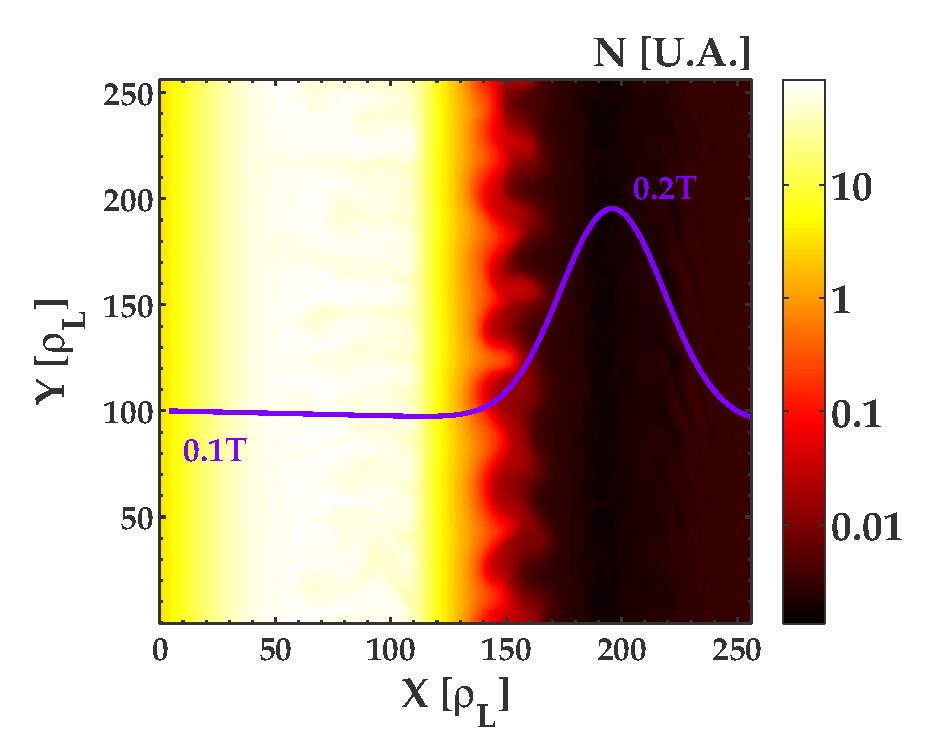
\includegraphics[height=5.8cm]{figures/2-CarteDensiteMagBarrier.eps}}
    \subfigure[]{\label{2-CartePotentielMagBarrier}
    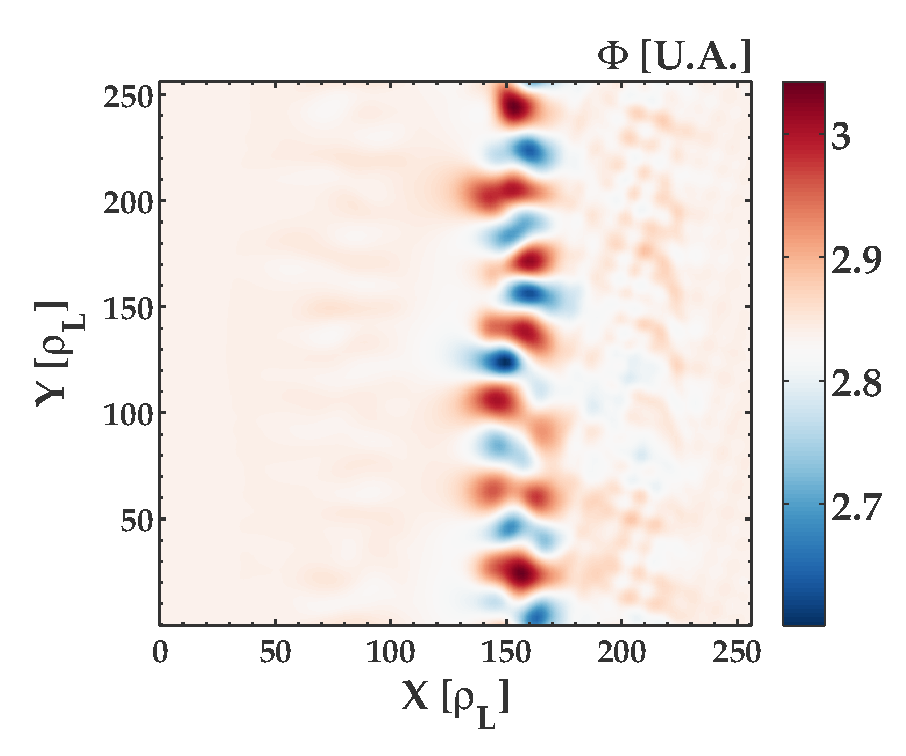
\includegraphics[height=5.8cm]{figures/2-CartePotentielMagBarrier.eps}}
    \caption{Cartes de densité \subref{2-CarteDensiteMagBarrier} et de potentiel
    \subref{2-CartePotentielMagBarrier}}
    \label{2-CartesMagBarrier}
\end{figure}

On voit que la barrière est très efficace. La carte de densité, affichée avec
une échelle logarithme, montre des vaguelettes qui se déplacent rapidement
dans la direction poloïdale.
Au même endroit, le potentiel forme lui aussi des structures qui s'étalent le
long du gradient positif de champ magnétique. 
Dans cette simulation, c'est le cisaillement de cette vitesse de dérive qui
apparaît dans la direction poloïdale qui semble responsable de l'effet de
barrière. 


	\subsection{Implémentation de l'équation d'énergie}
	La fermeture isotherme choisie dans le modèle de TOKAM2D est aussi très
	discutable. Comme le potentiel plasma est fortement lié à la température
	électronique à travers les conditions de gaines, il a tendance à suivre ses
	fluctuations. Le transport transverse dans la SOL peut alors se voir grandement
	impacté par l'apparition d'un gradient radial de température qui donne
	naturellement naissance à une dérive poloïdale. De plus, la prise en compte des
	variations spatiales de la température complexifie énormément la relation de
	dispersion obtenue par analyse linéaire du modèle, et peut donner lieu à
	l'apparition d'instabilités différentes de l'interchange.
	
	Pour obtenir l'équation de la température électronique, nous partons de
	l'équation de conservation de l'énergie normalisée :
	
	\begin{equation} 
	\label{2-eqTempBase}
		\frac{3}{2}\partial_t \text{P}_e +
		\nabla\cdot\left(\frac{3}{2}\text{P}_e\mathbf{U}_e+\mathbf{Q}_e\right) +
		\text{P}_e\nabla\cdot\mathbf{U}_e=\mathcal{S}_{\text{T}_e} 
	\end{equation}
	
	avec $\text{P}_e=\text{NT}_e$ la pression électronique, $\mathbf{Q_e}$ le
	flux de chaleur normalisé et $\mathcal{S}_{\text{T}_e}$ un terme source
	d'énergie cohérent avec le flux entrant de particules. 
	
	Pour simplifier l'équation~\ref{2-eqTempBase}, et pour les mêmes
	considérations que précédemment, la vitesse fluide dans les divergences est
	prise égale à la vitesse de dérive électrique $\mathbf U_e=\mathbf
	U_\text{E}$. La direction parallèle apparaît à travers un terme de
	perte qui représente la quantité d'énergie portée par le flux d'électrons
	perdue dans la gaine.
	Le flux de chaleur est choisi proportionnel au gradient de pression\footnote{Plusieurs expressions
	sont utilisées pour décrire la divergence du flux de chaleur. Le plus souvent,
	on choisit un terme proportionnel au gradient de température 
$\mathbf{Q}=\chi\nabla\text{T}_e$. Dans
notre modèle $\mathbf{Q}=\chi\nabla\text{P}_e$ pour ajouter un terme diffusif
analogue à celui des deux autres équations.} $\mathbf{Q}=\chi\nabla\text{P}_e$
afin contrôler l'amplitude des flux diffusifs dans la direction perpendiculaire.
	Les équations du modèle s'écrivent alors :
	
%\hspace*{-2cm}\begin{minipage}{1.1\textwidth}
\begin{align}
\label{2-eqContinuiteTemp}
\partial_t \text{N}
=& - \nabla\cdot\left(\text{N}\mathbf U_\text{E}\right) -\sigma
\text{N}\sqrt{\text{T}_e}e^{\Lambda-\Delta\Phi/\text{T}_e} + D\nabla^2 \text{N}
+ \mathcal{S}
\\[0.5cm]
\label{2-eqCourantTemp}
\begin{split}
\partial_{t}\text{W} =& 
-\nabla\cdot\left(\text{W}\mathbf U_\text{E}\right)
+\text{B}^2\sigma\sqrt{\text{T}_e}\left(1-e^{\Lambda-\Delta\Phi/\text{T}_e}\right)\\
&-\text{B}^2\nabla\cdot\left(\text{N}\mathbf
U_{\nabla\text{B}}\right)/\text{N} +\nu\nabla^2\text{W}
\end{split}
\\[0.5cm]
\label{2-eqEnergyTemp}
\begin{split}
\partial_{t}\text{P}_e=&
-\nabla\cdot\left(\text{P}_e\mathbf U_\text{E}\right)
+2/3\left(\gamma\sigma\text{P}_e\sqrt{\text{T}_e}e^{\Lambda-\Delta\Phi/\text{T}_e}\right.\\
&\left.-\text{P}_e\nabla\cdot\mathbf U_\text{E}
+\chi\nabla^2\text{P}_e
+\mathcal{S}_{\text{T}_e}\right)
\end{split}
\end{align}

%\end{minipage}

avec $\gamma$ un coefficient pris égal à 5/2. 
\subsubsection{Impact sur le transport transverse}

La figure~\ref{2-CartesWithTe} montre les solutions calculées par TOKAM2D avec
la température électronique dans une géométrie mono-périodique. On remarque tout
de suite que les trois champs sont fortement corrélés : pour la densité et
la température, ce n'est pas surprenant, les équations qui gouvernent leur
évolution sont très similaires. 
\begin{figure}[!htbp]
    \centering
    \subfigure[]{\label{2-CarteDensiteWithTe}
    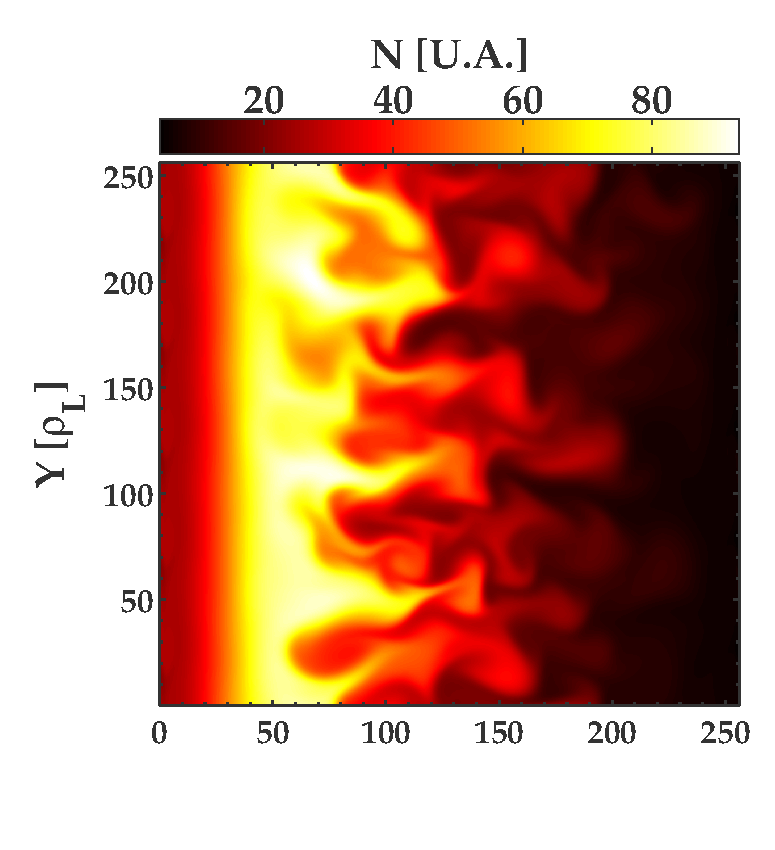
\includegraphics[height=5.75cm]{figures/2-CarteDensiteWhTe.eps}}
    \subfigure[]{\label{2-CartePotentielWithTe}
    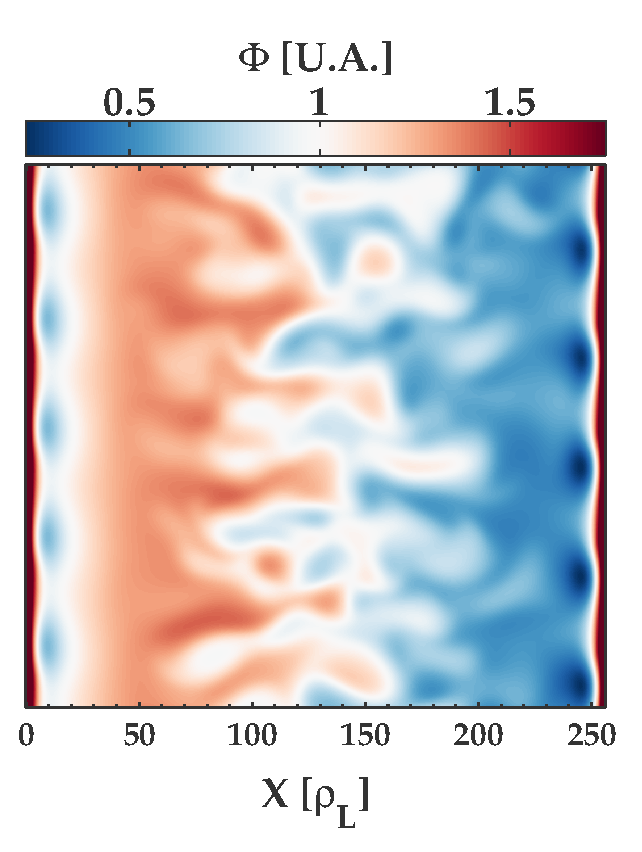
\includegraphics[height=5.75cm]{figures/2-CartePotentielWhTe.eps}}
    \subfigure[]{\label{2-CarteTeWhTe}
    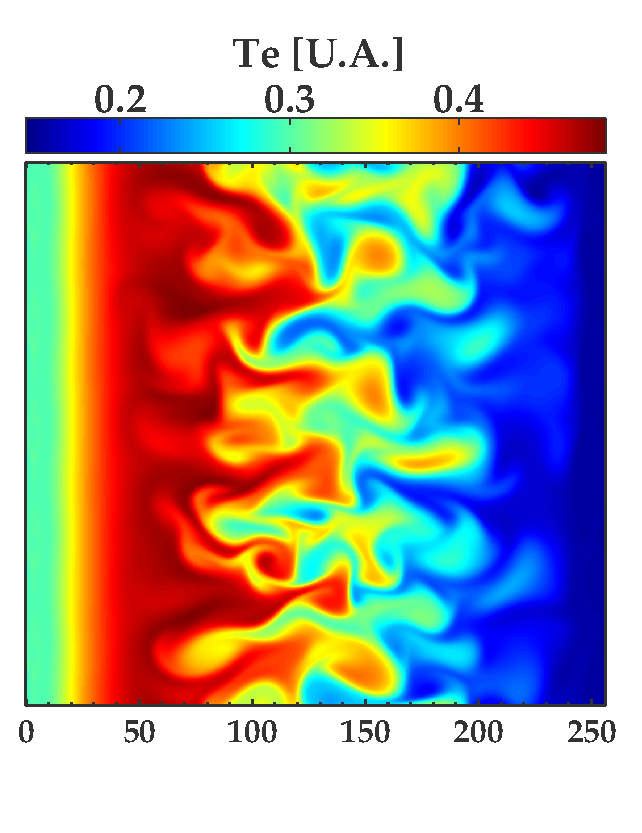
\includegraphics[height=5.75cm]{figures/2-CarteTeWhTe.eps}}
    \caption{Cartes de densité~\subref{2-CarteDensiteWithTe}~, de
    potentiel~\subref{2-CartePotentielWithTe}~ et de température 
    électronique~\subref{2-CarteTeWhTe}~.}
    \label{2-CartesWithTe}
	\end{figure}
	
Le potentiel ne forme plus de structures aussi
distinctives mais a lui aussi
plutôt tendance à suivre les fluctuations de température. En effet,
contrairement aux simulations isothermes, le potentiel flottant $\Phi_s$ défini
par $j_\para=\,$0 n'est plus constant mais dépend spatialement de la
température électronique :

\begin{equation}
	\Phi_{s}=\Lambda\text{T}_e(x,y)
\end{equation}

La figure~\ref{2-CartePotentielSurTeWhTedNdx} montre le rapport
$\Phi/\text{T}_e$, intervenant dans les conditions aux limites parallèles. Ce
rapport étant centré autour de $\Lambda$, on constate que le transport du
courant dans la direction parallèle force le potentiel à suivre les
variations de température en rappellant de façon exponentielle le potentiel
plasma à $\Lambda\text{T}_e$. Il est donc déterminant dans l'équilibre qui
se met en place.

\begin{figure}[!htbp]
\centering
	\subfigure[]{\label{2-CartePotentielSurTeWhTedNdx}
    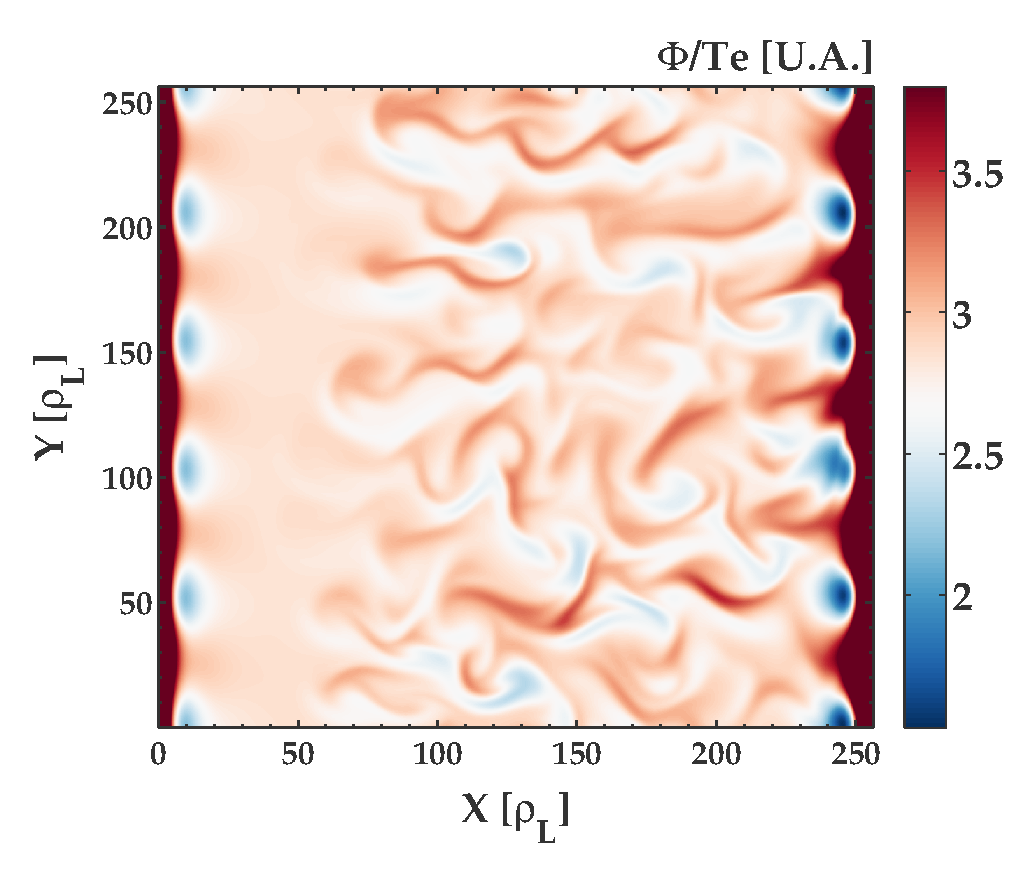
\includegraphics[height=6cm]{figures/2-CartePotentielSurTeWhTedNdx.eps}}
	\subfigure[]{\label{2-ProfileFluxWhTe}
    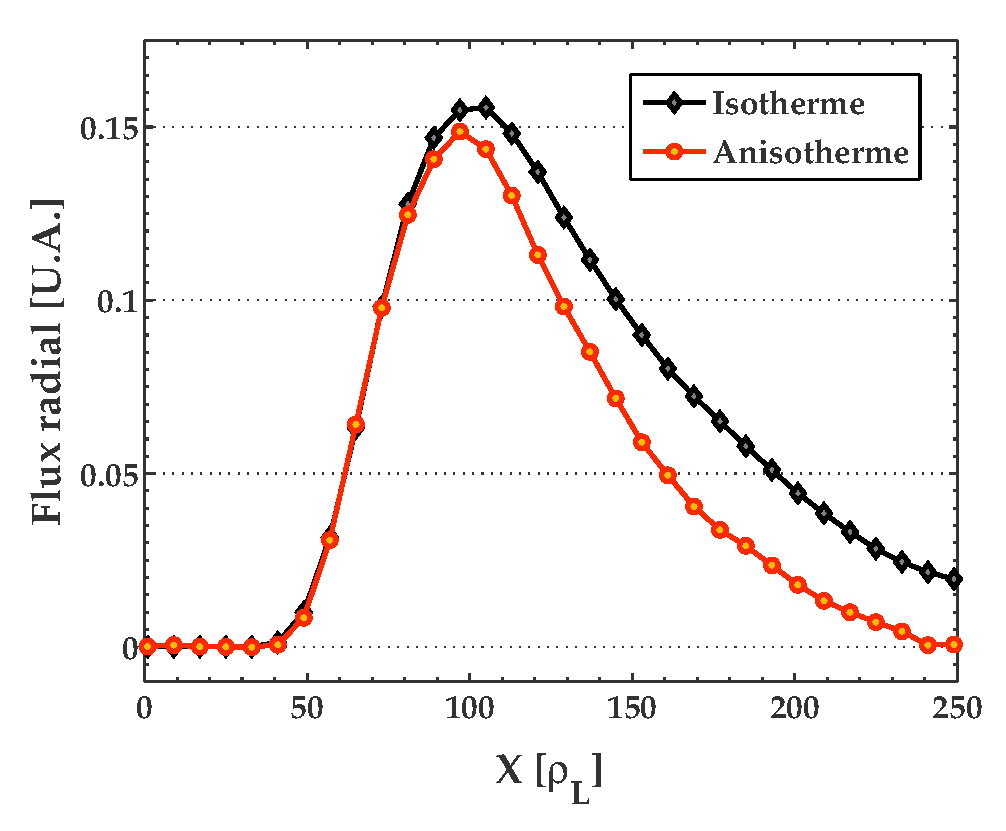
\includegraphics[height=5.5cm]{figures/2-profileFluxRadialWhTedNdx.eps}}    
    \caption{\subref{2-CartePotentielSurTeWhTedNdx}~ Carte du potentiel électrostatique
    rapporté à la température. \subref{2-ProfileFluxWhTe}~~Comparaison des
    profils du flux radial moyenné poloïdalement entre les cas isotherme et
    anisothermes.}
\end{figure}

L'une des conséquences immédiatement observables de cette corrélation est
l'apparition d'un champ électrique radial moyen non nul, qui, combiné au champ
magnétique, donne naissance à une dérive poloïdale du type ExB. Sur la
figure~\ref{2-ProfileFluxWhTe}, on peut voir que par rapport au cas isotherme,
le transport transverse est réduit notablement. En observant la dynamique
des flux, on voit que cette diminution est reliée au cisaillement créé par la
variation de cette dérive, dont l'intensité change en fonction du gradient de
potentiel, lui même proche du gradient de température.

Ce phénomène rappelle les "zonal flows" qui se forment en présence
d'un champ électrique radial $\nabla_x{\Phi}$. Pour illustration, les profils
moyennés en temps et en $y$ du potentiel électrique, du flux radial et du
flux poloïdal sont montés figure~\ref{2-profileFluxRadialWhTedNdx}. On y voit que le flux poloïdal moyen
est plus important que son homologue radial, mais surtout qu'il suit
le gradient radial de potentiel (positif quand $\nabla_x\Phi\ge\,$0 et négatif
quand $\nabla_x\Phi<\,$0), confirmant l'hypothèse proposée pour son origine.

	\begin{figure}[!htbp]
    \centering
    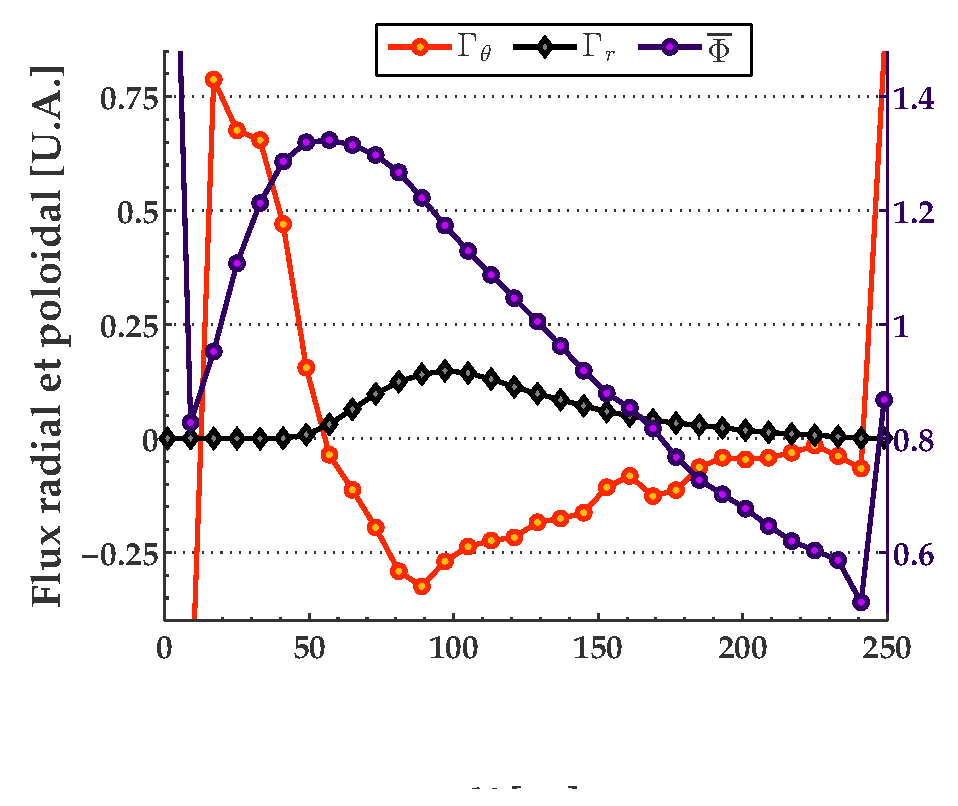
\includegraphics[height=6cm]{figures/2-profileFluxWhTedNdx.eps}
    \caption{Profils dans la direction radiale du potentiel moyen
    $\left<\Phi\right>_{t,y}$ et du flux poloïdal $\left<\Gamma_y\right>_{t,y}$
    généré, à comparer avec le flux radial moyen
    $\left<\Gamma_x\right>_{t,y}$.\label{2-profileFluxRadialWhTedNdx}}
	\end{figure}

Le dernier point intéressant à relever se voit le long des parois, où une
instabilité de type Kelvin-Helmholtz se développe. Le potentiel, décroissant de
la source aux parois, est fixé artificiellement à $\Lambda$ au niveau de la gaine.
Là encore, le champ électrique qui émerge à proximité immédiate de la limite du
domaine donne naissance à une dérive poloïdale qui varie sur une très courte
distance, se cisaille et génère des vortex caractéristiques de l'instabilité.
Les travaux réalisés par Theilhaber sur la modélisation PIC 2D de l'interaction
plasma-surface perpendiculairement au champ magnétique
\parencite{Theilhaber} montrent que l'instabilité de Kelvin-Helmotz est à
l'origine de la formation d'une gaine "de champs croisés" de largeur $l\sim\,$
5$\,\rho_{Li}$.

Dans cette simulation, ce phénomène est un artefact des
conditions aux limites strictes. On peut toutefois imaginer que si un fort
champ électrique se forme en face de la paroi (comme celui de la gaine), tout
flux arrivant sera dévié perpendiculairement par effet de dérive.
Dans les sources d'ions avec barrière magnétique, ce comportement peut être
observé à proximité des parois dans la région du filtre, mais est encore assez
mal compris.
Il rappelle cependant que le choix des conditions aux limites dans la direction
transverse n'est pas sans conséquences sur le transport et qu'une théorie
serait nécessaire pour décrire convenablement le transport.

Nous illustrons maintenant l'ajout de la température par deux exemples, la
barrière magnétique que nous avons regardée précédemment et une colonne de
plasma, où le transport devient turbulent malgré un champ magnétique uniforme, ce qui
n'était pas le cas avec une hypothèse isotherme.

	\subsubsection{Application au filtre magnétique}

Nous reprenons les paramètres de simulation de la barrière magnétique, mais en
incluant l'évolution de la température électronique. Les cartes des trois champs
sont présentées sur les figures~\ref{2-CartesWithTeFiltre}. Le
potentiel électrostatique suit toujours les variations de température, ce qui
provoque l'apparition d'une dérive poloïdale, très cisaillée, et stoppe complètement le
transport des particules dans la direction radiale. Au parois, on observe le
même phénomène que précédemment ; il est dû là aussi aux conditions aux limites
transverses.

	\begin{figure}[!htbp]
    \centering
    \subfigure[]{\label{2-CarteDensiteMagBarrierWhTe}
    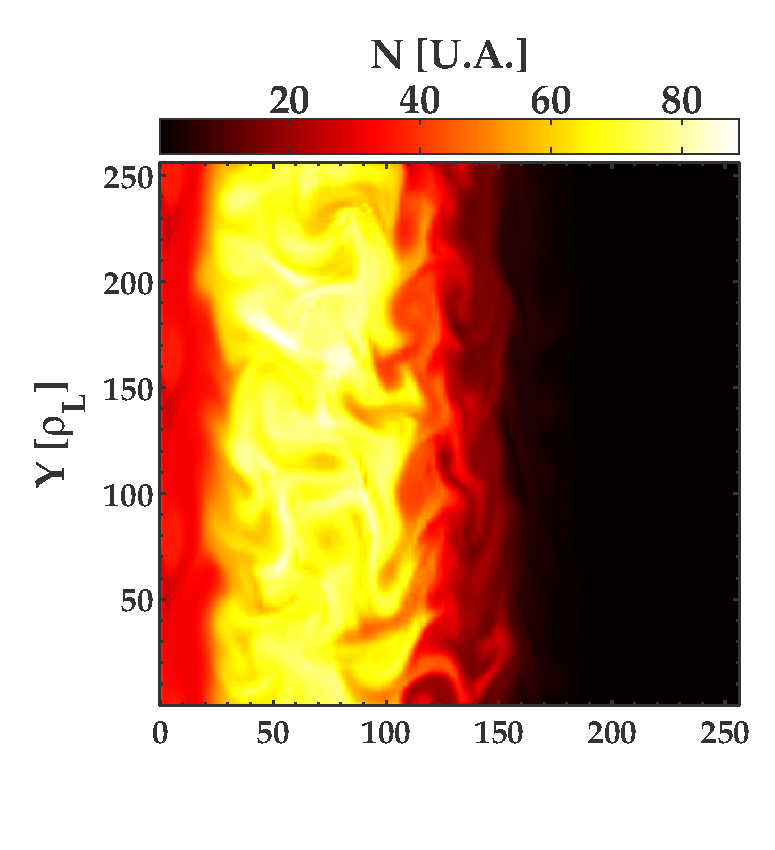
\includegraphics[height=5.75cm]{figures/2-CarteDensiteMagBarrierWhTe.eps}}
    \subfigure[]{\label{2-CartePotentielMagBarrierWhTe}
    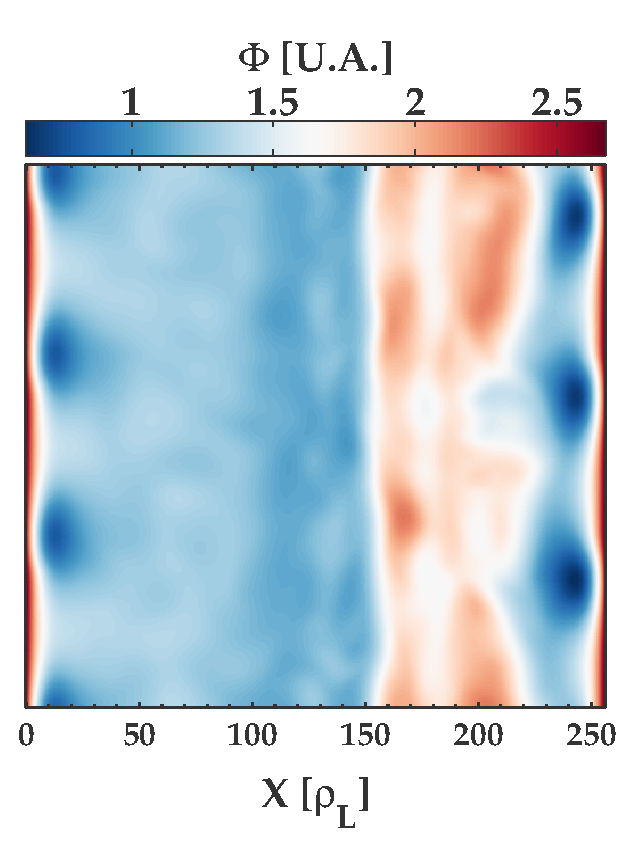
\includegraphics[height=5.75cm]{figures/2-CartePotentielMagBarrierWhTe.eps}}
    \subfigure[]{\label{2-CarteTeMagBarrierWhTe}
    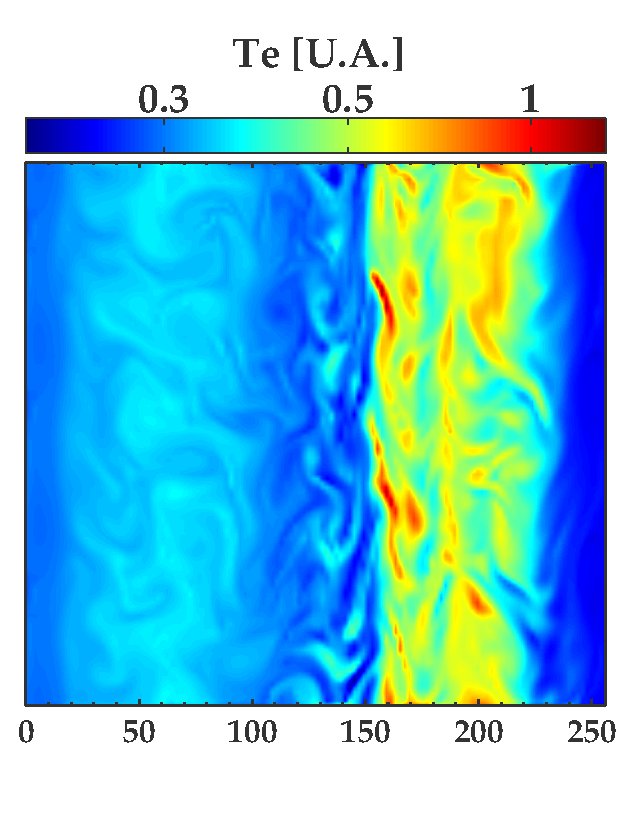
\includegraphics[height=5.75cm]{figures/2-CarteTeMagBarrierWhTe.eps}}
    \caption{Cartes de densité~\subref{2-CarteDensiteMagBarrierWhTe}~, de
    potentiel~\subref{2-CartePotentielMagBarrierWhTe}~et de température
   \subref{2-CarteTeMagBarrierWhTe}~.}
    \label{2-CartesWithTeFiltre}
	\end{figure}
	
Contrairement au cas des plasmas froids, où les électrons perdent leur énergie
par collision dans le piège magnétique, on
remarque que dans cette simulation la température croît avec
l'intensité du champ. Sur la carte de température, on voit bien l'emplacement du
zonal flow au niveau du gradient de potentiel, en $x\sim\,$140$\,\rho_{Li}$.
	
\subsubsection{Simulation d'une colonne de plasma magnétisée}
Regardons maintenant une configuration de type colonne magnétisée : 

\begin{itemize}
  \item le champ magnétique est pris homogène et constant, d'intensité B = 0.1~T
  \item les dimensions de la source sont prises égales à 16 cm x
  16 cm x 6 m, avec un rayon
  de Larmor ionique $\rho_{Li}\simeq$~6~10$^{-4}$~m et une conductivité
  parallèle $\sigma=\rho_{Li}/L_\para=\,$10$^{-4}$
  \item à la paroi, dans la direction perpendiculaire au champ magnétique, le
  potentiel plasma est fixé au potentiel flottant $\Lambda$
  \item une source de particules, avec un profil gaussien de largeur
  $l_{\mathcal S}=\,$32$\,\rho_{Li}$, est placée au centre du domaine
\end{itemize}

Les simulations isothermes de cette configuration sont stationnaires : la
densité et le potentiel électrostatique sont décroissants du centre de la
source jusqu'aux parois. 

Quand la température électronique est prise en compte,
le plasma commence à se déformer et une instabilité, indépendante de la
courbure du champ magnétique, se développe.
La caractérisation de cette instabilité est encore à réaliser
mais on peut dores et déjà essayer de la relier au travaux
réalisés dans~\parencite{Berk} qui prédisent une instabilité à fort taux de
croissance en présence de parois conductrice et d'un gradient de température.
Conformément à nos attentes, le plasma est en rotation dans le plan transverse (sur les
figures~\ref{2-MagColumnWithTe}, la rotation s'effectue dans le sens
anti-trigonométrique, qui correspond à la direction de la dérive ExB).

Les conditions aux limites choisies, en supposant $\Phi=\Lambda$ et $W=0$ à la
paroi, empêche le courant de rentrer ou de sortir par les bords latéraux. Comme
les électrons sont moins mobiles que les ions perpendiculairement au champ
magnétique, pour conserver
la quasineutralité du plasma, le courant préfère passer le long des lignes de
champ, court-circuitant le transport perpendiculaire.

 \begin{figure}[!htbp]
    \centering
    \subfigure[]{\label{2-CarteDensiteMagColumn}
    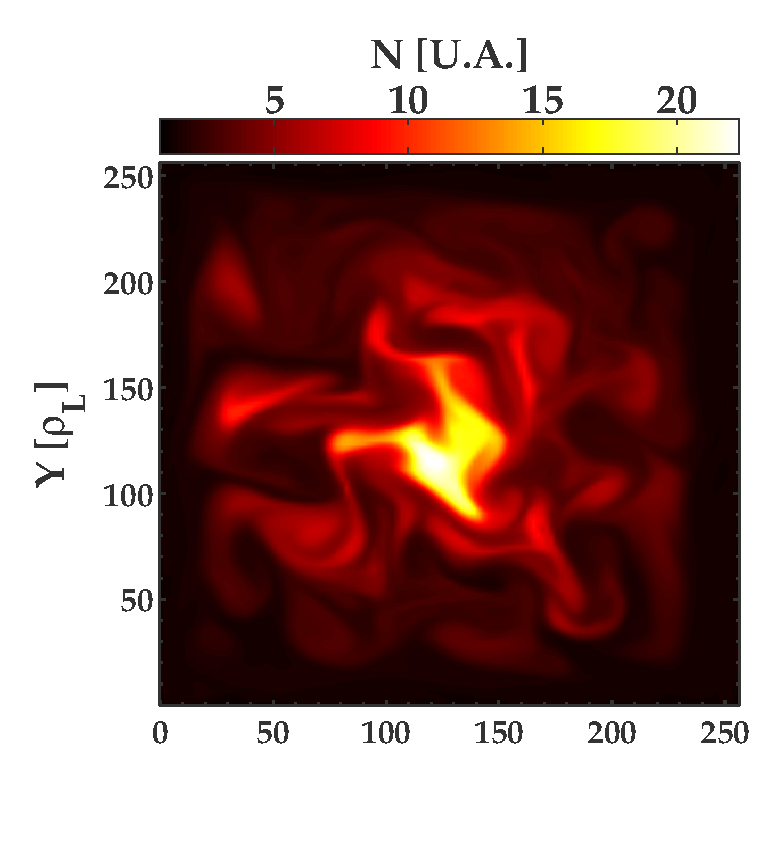
\includegraphics[height=5.75cm]{figures/2-CarteDensiteMagColumn.eps}}
    \subfigure[]{\label{2-CartePotentielMagColumn}
    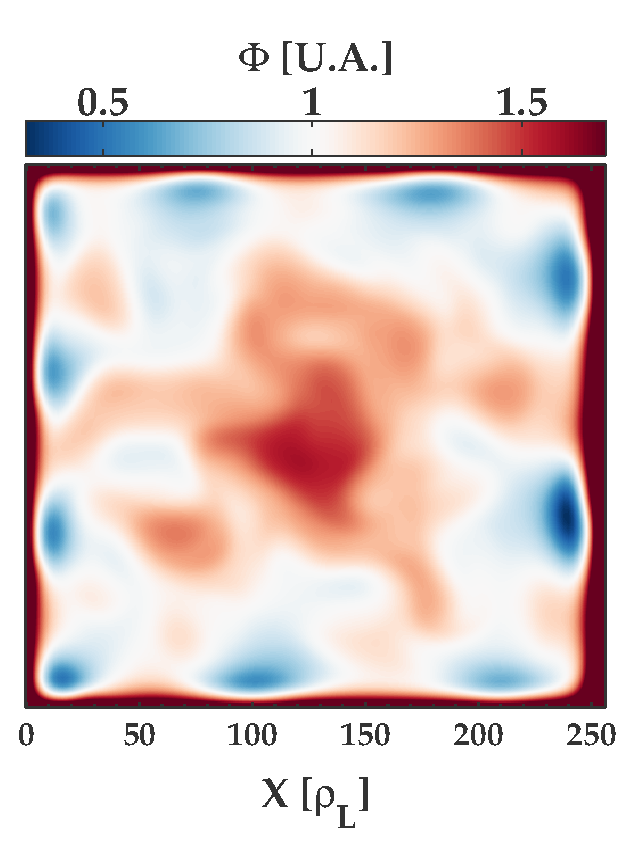
\includegraphics[height=5.75cm]{figures/2-CartePotentielMagColumn.eps}}
    \subfigure[]{\label{2-CarteTeMagColumn}
    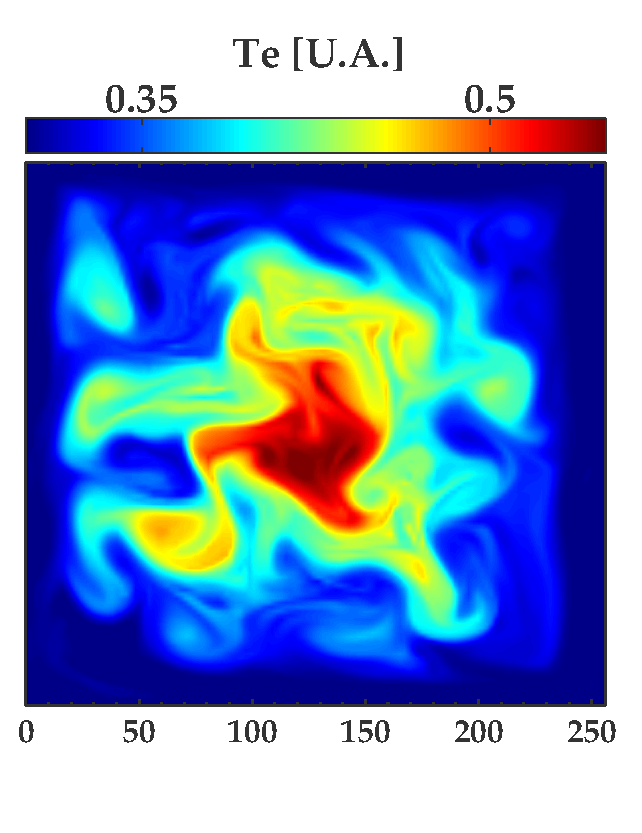
\includegraphics[height=5.75cm]{figures/2-CarteTeMagColumn.eps}}
    \caption{Cartes de densité \subref{2-CarteDensiteMagColumn}, de potentiel
    \subref{2-CartePotentielMagColumn} et de température \subref{2-CarteTeMagColumn}}
    \label{2-MagColumnWithTe}
	\end{figure}
	
\section{L'approche par vitesses de dérive pour les plasmas
froids}
\label{vitessesDerivePlasmaFroid}
\parencite{Sudan}
Les équations de TOKAM2D ne décrivent
pas non plus l'interaction collisionnelle des particules chargées avec la
population neutre, essentielle dans la physique des plasmas froids. Dans les
régions non magnétisées, l'hypothèse de forte magnétisation sur laquelle se
base l'approximation des vitesses de dérive n'est plus valable. Pour étendre le
domaine de validité du modèle, on peut cependant dériver une nouvelle
expression des vitesses de dérive qui tient alors compte de l'interaction
avec les neutres. Les équations forment une sorte de combinaison entre les
équations du transport magnétisé et celles du modèle de dérive-diffusion.

Reprenons l'équation du moment pour une espèce d'indice $\alpha$ :

\begin{equation}
\label{2-MaplEqMoment}
\frac{\text{d}\mathbf{u}_\alpha}{\text{dt}}+
\nu_\alpha\mathbf{u}_\alpha+\omega_{c\alpha}\mathbf{b}\times\mathbf{u}_\alpha=
-\frac{q_\alpha}{m_\alpha}\left(\nabla \Phi +\frac{\nabla p_\alpha}{q_\alpha n_\alpha}\right)
\end{equation}

En prenant le produit vectoriel de \eqref{2-MaplEqMoment} et du champ
magnétique,  on peut éliminer le terme de
Lorentz $\omega_{c\alpha}\mathbf{b}\times\mathbf{u}_\alpha$ :

\begin{equation}
\label{2-MaplVitesse}
\mathbf{u}_\alpha=\frac{q_\alpha}{m_\alpha}(\nu_\alpha\puissance{2b}+\omega_{c\alpha}\puissance{2})\puissance{-1}
-\frac{q_\alpha}{m_\alpha}\left(\nabla \Phi +\frac{\nabla p_\alpha}{q_\alpha
n_\alpha}\right)-\frac{\text{d}\mathbf{u}_\alpha}{\text{dt}}
\end{equation}

 \begin{figure}[!htbp]
    \centering
    \subfigure[]{\label{2-CarteDensiteMapl}
    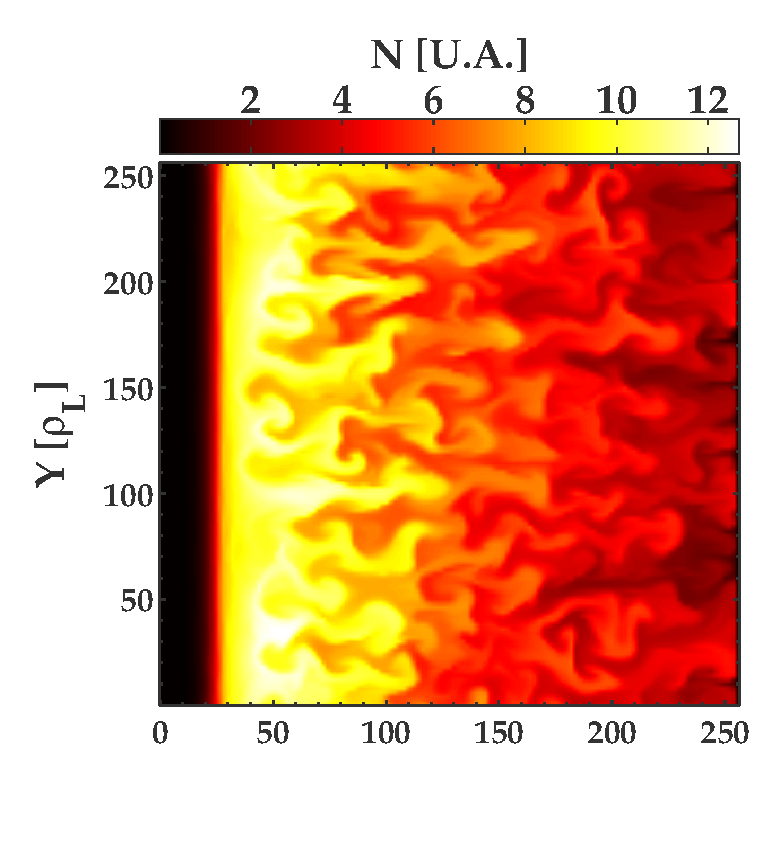
\includegraphics[height=8cm]{figures/2-CarteDensiteMapl.eps}}
    \subfigure[]{\label{2-CartePotentielMapl}
    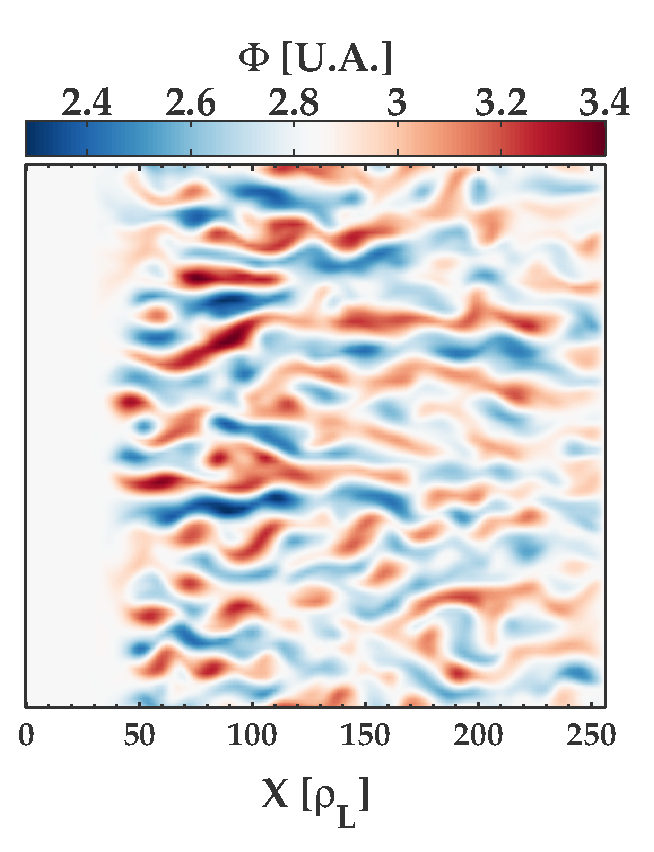
\includegraphics[height=8cm]{figures/2-CartePotentielMapl.eps}}
    \caption{Cartes de densité \subref{2-CarteDensiteMapl}~~et de potentiel
    \subref{2-CartePotentielMapl}}
	\end{figure}
%\bibliographystyle{apalike}
%\bibliography{biblio}

\end{refsection}




